\documentclass[pdf]{beamer}
\mode<presentation>{
\usetheme{Ilmenau}

}
\usecolortheme{dolphin}
\usepackage[UTF8,indent]{ctexcap}
\usepackage{amssymb}
\usepackage{amsmath}
\usepackage{amsfonts}
%\usepackage{graphicx}
\usepackage{amsthm}
\usepackage{indentfirst}
\usepackage{enumerate}
\usepackage{extpfeil}
\usepackage{tikz-cd}

%\usepackage{xmpmulti}

\usetikzlibrary {calc,positioning,shapes.misc,graphs,decorations.pathreplacing}
\usefonttheme[onlymath]{serif}

\numberwithin{equation}{section}

\theoremstyle{plain}
\newtheorem{proposition}[theorem]{Proposition}
\newtheorem{claim}[theorem]{Claim}
\newtheorem{defn}[theorem]{Definition}

\theoremstyle{plain}
\newtheorem{exercise}{Exercise}[section]


\theoremstyle{remark}
\newtheorem{remark}[theorem]{Remark}
\newtheorem{remarks}{Remarks}
\newtheorem{ex}[theorem]{Exercise}
\newtheorem{question}[theorem]{Question}

\DeclareMathOperator{\Id}{\operatorname{Id}}
\DeclareMathOperator{\supp}{supp}
\DeclareMathOperator{\dist}{dist}
\DeclareMathOperator{\vol}{vol}
\DeclareMathOperator{\diag}{diag}
\DeclareMathOperator{\tr}{tr}
\DeclareMathOperator{\divi}{\operatorname{div}}
\DeclareMathOperator{\cha}{\operatorname{char}}
\DeclareMathOperator{\Proj}{\operatorname{Proj}}
\DeclareMathOperator{\rank}{\operatorname{rank}}
\DeclareMathOperator{\Ker}{\operatorname{Ker}}
\DeclareMathOperator{\coker}{\operatorname{Coker}}
\DeclareMathOperator{\Img}{\operatorname{Im}}
\DeclareMathOperator{\tor}{\operatorname{tor}}
\DeclareMathOperator{\prim}{\operatorname{prim}}
\DeclareMathOperator{\Perm}{\operatorname{Perm}}

\newcommand{\Hom}{\operatorname{Hom}}
\newcommand{\Ext}{\operatorname{Ext}}
\newcommand{\Spec}{\operatorname{Spec}}
\newcommand{\Pic}{\operatorname{Pic}}
\newcommand{\Jac}{\operatorname{Jac}}
\newcommand{\MaxSpec}{\operatorname{MaxSpec}}
\newcommand{\End}{\operatorname{End}}
\newcommand{\Mod}{\operatorname{\textbf{Mod}}}
\newcommand{\Gal}{\operatorname{Gal}}
\newcommand{\Aut}{\operatorname{Aut}}
\newcommand{\Grp}{\operatorname{\textbf{Grp}}}
\newcommand{\Set}{\operatorname{\textbf{Set}}}
\newcommand{\Stab}{\operatorname{Stab}}
\newcommand{\ord}{\operatorname{ord}}
\newcommand{\PSL}{\operatorname{\mathbb{P}SL}}



\newcommand*{\bigchi}{\mbox{\Large$\chi$}}% big chi
\setlength{\parindent}{2em}
\newcommand{\character}[2]{\left[\begin{array}{c}{#1} \\ {#2}\end{array}\right]}
\newcommand{\normalcharacter}{\character{\epsilon}{\epsilon'}}

\setbeamertemplate{caption}[numbered]
% 设置图形文件的搜索路径
\graphicspath{{figures/}}
\title{本科毕业论文答辩}
\author{周潇翔}
\institute[USTC]{University of Science and Technology of China}
\date{\today}
\subject{模形式和五次方程的解}
\keywords{正多面体,\enskip 分歧覆叠,\enskip 预解式,\enskip 求根公式,\enskip 模形式,\enskip Theta函数,\enskip Klein四次曲线}
\tikzset{
invisible/.style={opacity=0,text opacity=0},
visible on/.style={alt=#1{}{invisible}},
alt/.code args={<#1>#2#3}{%
\alt<#1>{\pgfkeysalso{#2}}{\pgfkeysalso{#3}} % \pgfkeysalso doesn't change the path
},
}
\begin{document}
\setbeamercovered{transparent}
\begin{frame}{正多面体方程}
	\begin{table}[ht]
	\centering
	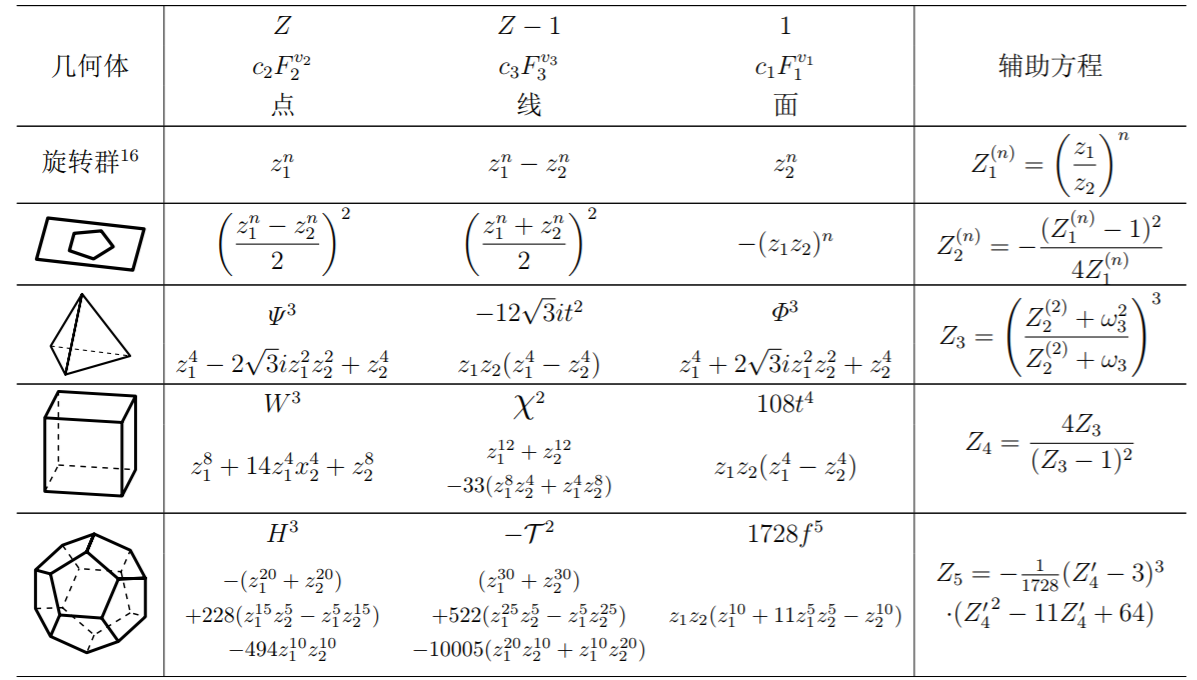
\includegraphics[width=0.9\textwidth]{snip/eqpoly.png}
	\caption{正多面体对应方程}
	\label{tb:equations}
\end{table}
\end{frame}

\begin{frame}{辅助方程}
	\begin{remarks}\
		\begin{enumerate}[1.]
			\item 由于嵌入正十二面体的立方体为倾斜放置,辅助方程为$Z_4'$,与$Z_4$相差一个分式线性变换.倾斜的立方体对应的$F_1,F_2,F_3$及其代数关系如下:
			\begin{figure}[ht]
				\centering
				\hspace{-1cm}
				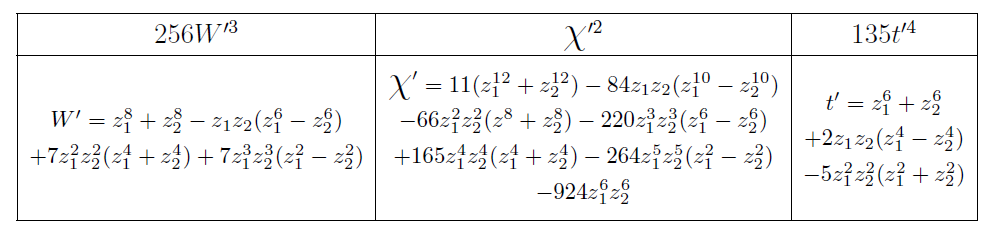
\includegraphics[width=0.98\textwidth]{snip/slantpoly.png}
			\end{figure}
			\item 通过辅助方程,除$Z_5(z)$以外的其他方程均可解出,且为根式解.但是正十二面体所对应的最后一个辅助方程是5次方程!
		\end{enumerate}
	\end{remarks}
\end{frame}

%\begin{frame}{群与域扩张}
%另外,我们有扩张与Galois群的反向对应:
%\[	\setcounter{MaxMatrixCols}{15}
%\begin{array}{ccccccccc|cc}
%\mathbb{C}(z) &\supseteq &\mathbb{C}(Z_1^{(2)}) &\supseteq &\mathbb{C}(Z_2^{(2)}) &\supseteq &\mathbb{C}(Z_3) &\supseteq  &\mathbb{C}(Z_4) =  \mathbb{C}(Z_4') &\supseteq  &\mathbb{C}(Z_5)\\[-0.45cm]
%&\underset{2}{}&&\underset{2}{}&&\underset{3}{}&&\underset{2}{}&&\underset{5}{}&\\
%\{1\} &\lhd &C_2 &\lhd &D_2  &\lhd &A_4 &\lhd &S_4 &\leqslant &S_5
%\end{array}
%\]
%竖线左边为根式扩张与正规子群序列的对应,右边为非循环单群($\Rightarrow$不可解群)与非分式扩张的对应.
%\end{frame}

\begin{frame}{预解式}
	\begin{defn}
		我们称$r \in K$相对于Galois扩张$K/k$的\textbf{预解式}(resolution)为$r$的最小多项式$R_{r,K/k}$.
	\end{defn}
假设预解式可解即相当于给出$r$的值。对$t'$齐次化,得到亚纯函数
$$u:=\frac{12f^2}{\mathcal{T}} \cdot t'$$
计算得到($Z_5':= \{1728(1-Z_5)\}^{-1}$)
$$R_{u,\mathbb{C}(Z_4)/\mathbb{C}(Z_5)}(T):=T^5-10Z_5'T^3+45{Z_5'}^2T-{Z_5'}^2$$
被称作\textbf{Brioschi预解式}.

\end{frame}
\begin{frame}{正二十面体方程$\Longleftrightarrow$解Brischi预解式}
	$\Leftarrow$: 固定$Z_5=\lambda_0$,若给出$R_{u,\mathbb{C}(Z_4)/\mathbb{C}(Z_5)}(T)=0$的一个解$T=u_0$,则得到
	$$Z_4'=\frac{t'^2}{f}=\frac{u^2\mathcal{T}^2}{144f^5}=12u^2(1-Z_5)$$
	从而依次解出$Z_4,Z_3,Z_2^{(2)},Z_1^{(2)},z$,得到方程$Z_5(z)=\lambda_0$的解.
	
	$\Rightarrow$:若给出正二十面体方程解,直接算出$u$即可。

\end{frame}
\begin{frame}{方法:Jerrard-Bring约化}
记$k=\mathbb{Q}[a_0,\ldots,a_4]$,设原方程为
$$f(x):=x^5+a_4x^4+a_3x^3+a_2x^2+a_1x+a_0=0$$
其根记为$r_i$.
对某个多项式$t(T) \in k[T] \; \big(\mod f(T)\big)$,我们得到新的五次方程
\begin{equation*}\label{eq:closetoBri}
q(T):=\prod_{i=1}^{5} (T-t(r_i))=T^5+d_1T^4+d_2T^3+d_3T^2+d_4T+d_5 \in k[T]
\end{equation*}

\end{frame}
\begin{frame}{消去$a_4,a_3$}
设原方程为
$$f(x):=x^5+a_4x^4+a_3x^3+a_2x^2+a_1x+a_0=0$$
通过设$x'=x+b_0$我们消去$a_4$,再通过设$x'=x^2+b_1x+b_0$消去$a_3$,得到
$$p(x)=x^5-\sigma_3\alpha x^2+\sigma_4 x-\sigma_5=0$$
\end{frame}
\begin{frame}{消去$a_4,a_3$}
设原方程为
$$f(x):=x^5+a_4x^4+a_3x^3+a_2x^2+a_1x+a_0=0$$
通过设$x'=x+b_0$我们消去$a_4$,再通过设$x'=x^2+b_1x+b_0$消去$a_3$,得到
$$p(x)=x^5-\sigma_3\alpha x^2+\sigma_4 x-\sigma_5=0$$
\end{frame}
\begin{frame}{$p(x)=0 \Longleftrightarrow $ Brioschi预解式}
设原方程为
$$p(T):=T^5-\sigma_3 T^2+\sigma_4 T -\sigma_5$$
通过定义特定的多项式$t(T) \in k[T] \; \big(\mod p(T)\big)$(可通过线性代数、结式、对称多项式的计算算出),我们得到新的五次方程
\begin{equation*}
q(T):=\prod_{i=1}^{5} (T-t(r_i))=T^5+d_3T^3+d_4T+d_5 \in k[T]
\end{equation*}
放缩后得到Brioschi预解式.
\end{frame}
\begin{frame}{例:$p(x)=x^5+2x^2+2x+1=0$}
对方程
$$p(x)=x^5+2x^2+2x+1=0$$
定义多项式$t(T)=510T^4+120T^3+240T^2+600T+960$,运用Jerrard-Bring约化,我们得到五次方程
\begin{equation*}
q(T)=T^5-1782000T^3+1428985800000T-636613173900000 =0
\end{equation*}
取$T'=\frac{2}{40095}T$,则方程化为
\begin{equation*}
T'^5-\frac{320}{72171}T'^3+\frac{5120}{578739249}T'-\frac{1024}{5208653241}=0
\end{equation*}
此即为$W=\frac{32}{72171}$的Brioschi预解式.
\end{frame}

%%%%%%%%%%%%%%%%%%%%%%%%%%%%%%%%%%%%%%%%%%%%%%%%%%%%%%%%%%%%%%%%%%%%%%%%%%




%%%%%%%%%%%%%%%%%%%%%%%%%%%%%%%%%%%%%%%%%%%%%%%%%%%%%%%%%%%%%%%%%%%%%%%%%%%%%%%%%%%%%%%%%%%%%%%





\end{document}




